\documentclass[]{article}
\usepackage{caption,subcaption,graphicx,float,url,amsmath,amssymb,tocloft}
\usepackage[hidelinks]{hyperref}
\usepackage[toc,acronym,nonumberlist]{glossaries}
\setacronymstyle{long-short}
\usepackage{glossaries-extra}
\graphicspath{{figs/}} 
\setlength{\cftsubsecindent}{0em}
\setlength{\cftsecnumwidth}{3em}
\setlength{\cftsubsecnumwidth}{3em}

%opening
\title{
	Notes from Origins of Life\\
	Week 6: Astrobiology \& General Theories of Life
}
\author{Simon Crase}

\makeglossaries
\renewcommand{\thesection}{6.\arabic{section}}

\loadglsentries{glossary-entries}

\renewcommand{\glstextformat}[1]{\textbf{\em #1}}

\begin{document}

\maketitle

\begin{abstract}
   These are my notes from the $6^{th}$ Week of the Santa Fe Institute Origins of Life Course\cite{sfi2019}. The course aims to push the field of Origins of Life research forward by bringing new and synthetic thinking to the question of how life emerged from an abiotic world.\\
   The content and images contained herein are the intellectual property of the Santa Fe Institute, with the exception of any errors in transcription, which are my own.
   These notes are distributed in the hope that they will be useful,
   but without any warranty, and without even the implied warranty of
   merchantability or fitness for a particular purpose. All feedback is welcome,
   but I don't necessarily undertake to do anything with it.

\end{abstract}

\setcounter{tocdepth}{2}
\tableofcontents

\listoffigures

\section{Introduction}

Lecturer: Chris Kempes

Ultimate goal is to provide a general theory of Life, one capable of uncovering the history we know about, but also bounding the possibilities for other types of life, and helping us recognize other forms of life. In this unit we'll discuss the search for life beyond Earth and how origins of life fits into this effort. We'll also discuss general evolutionary processes and abstract life. 

\section{Origins of Life and Astrobiology}

Lecturer: Sara Imari Walker

Why is Origins so important to Astrobiology? We want to be able to identify living organisms on another planet. We can send robotic missions within the Solar System, but we have only a small amount of data for exoplanets.

 What makes worlds with life different--Figure \ref{fig:Jupiter:Tellus}? Jupiter and Earth both have non-equilibrium surface features, so that isn't sufficient.

\begin{figure}[H]
	\caption{What makes worlds with life different?}\label{fig:Jupiter:Tellus}
	\begin{subfigure}[b]{0.45\textwidth}
		\caption{Jupiter}\label{fig:Jupiter}
		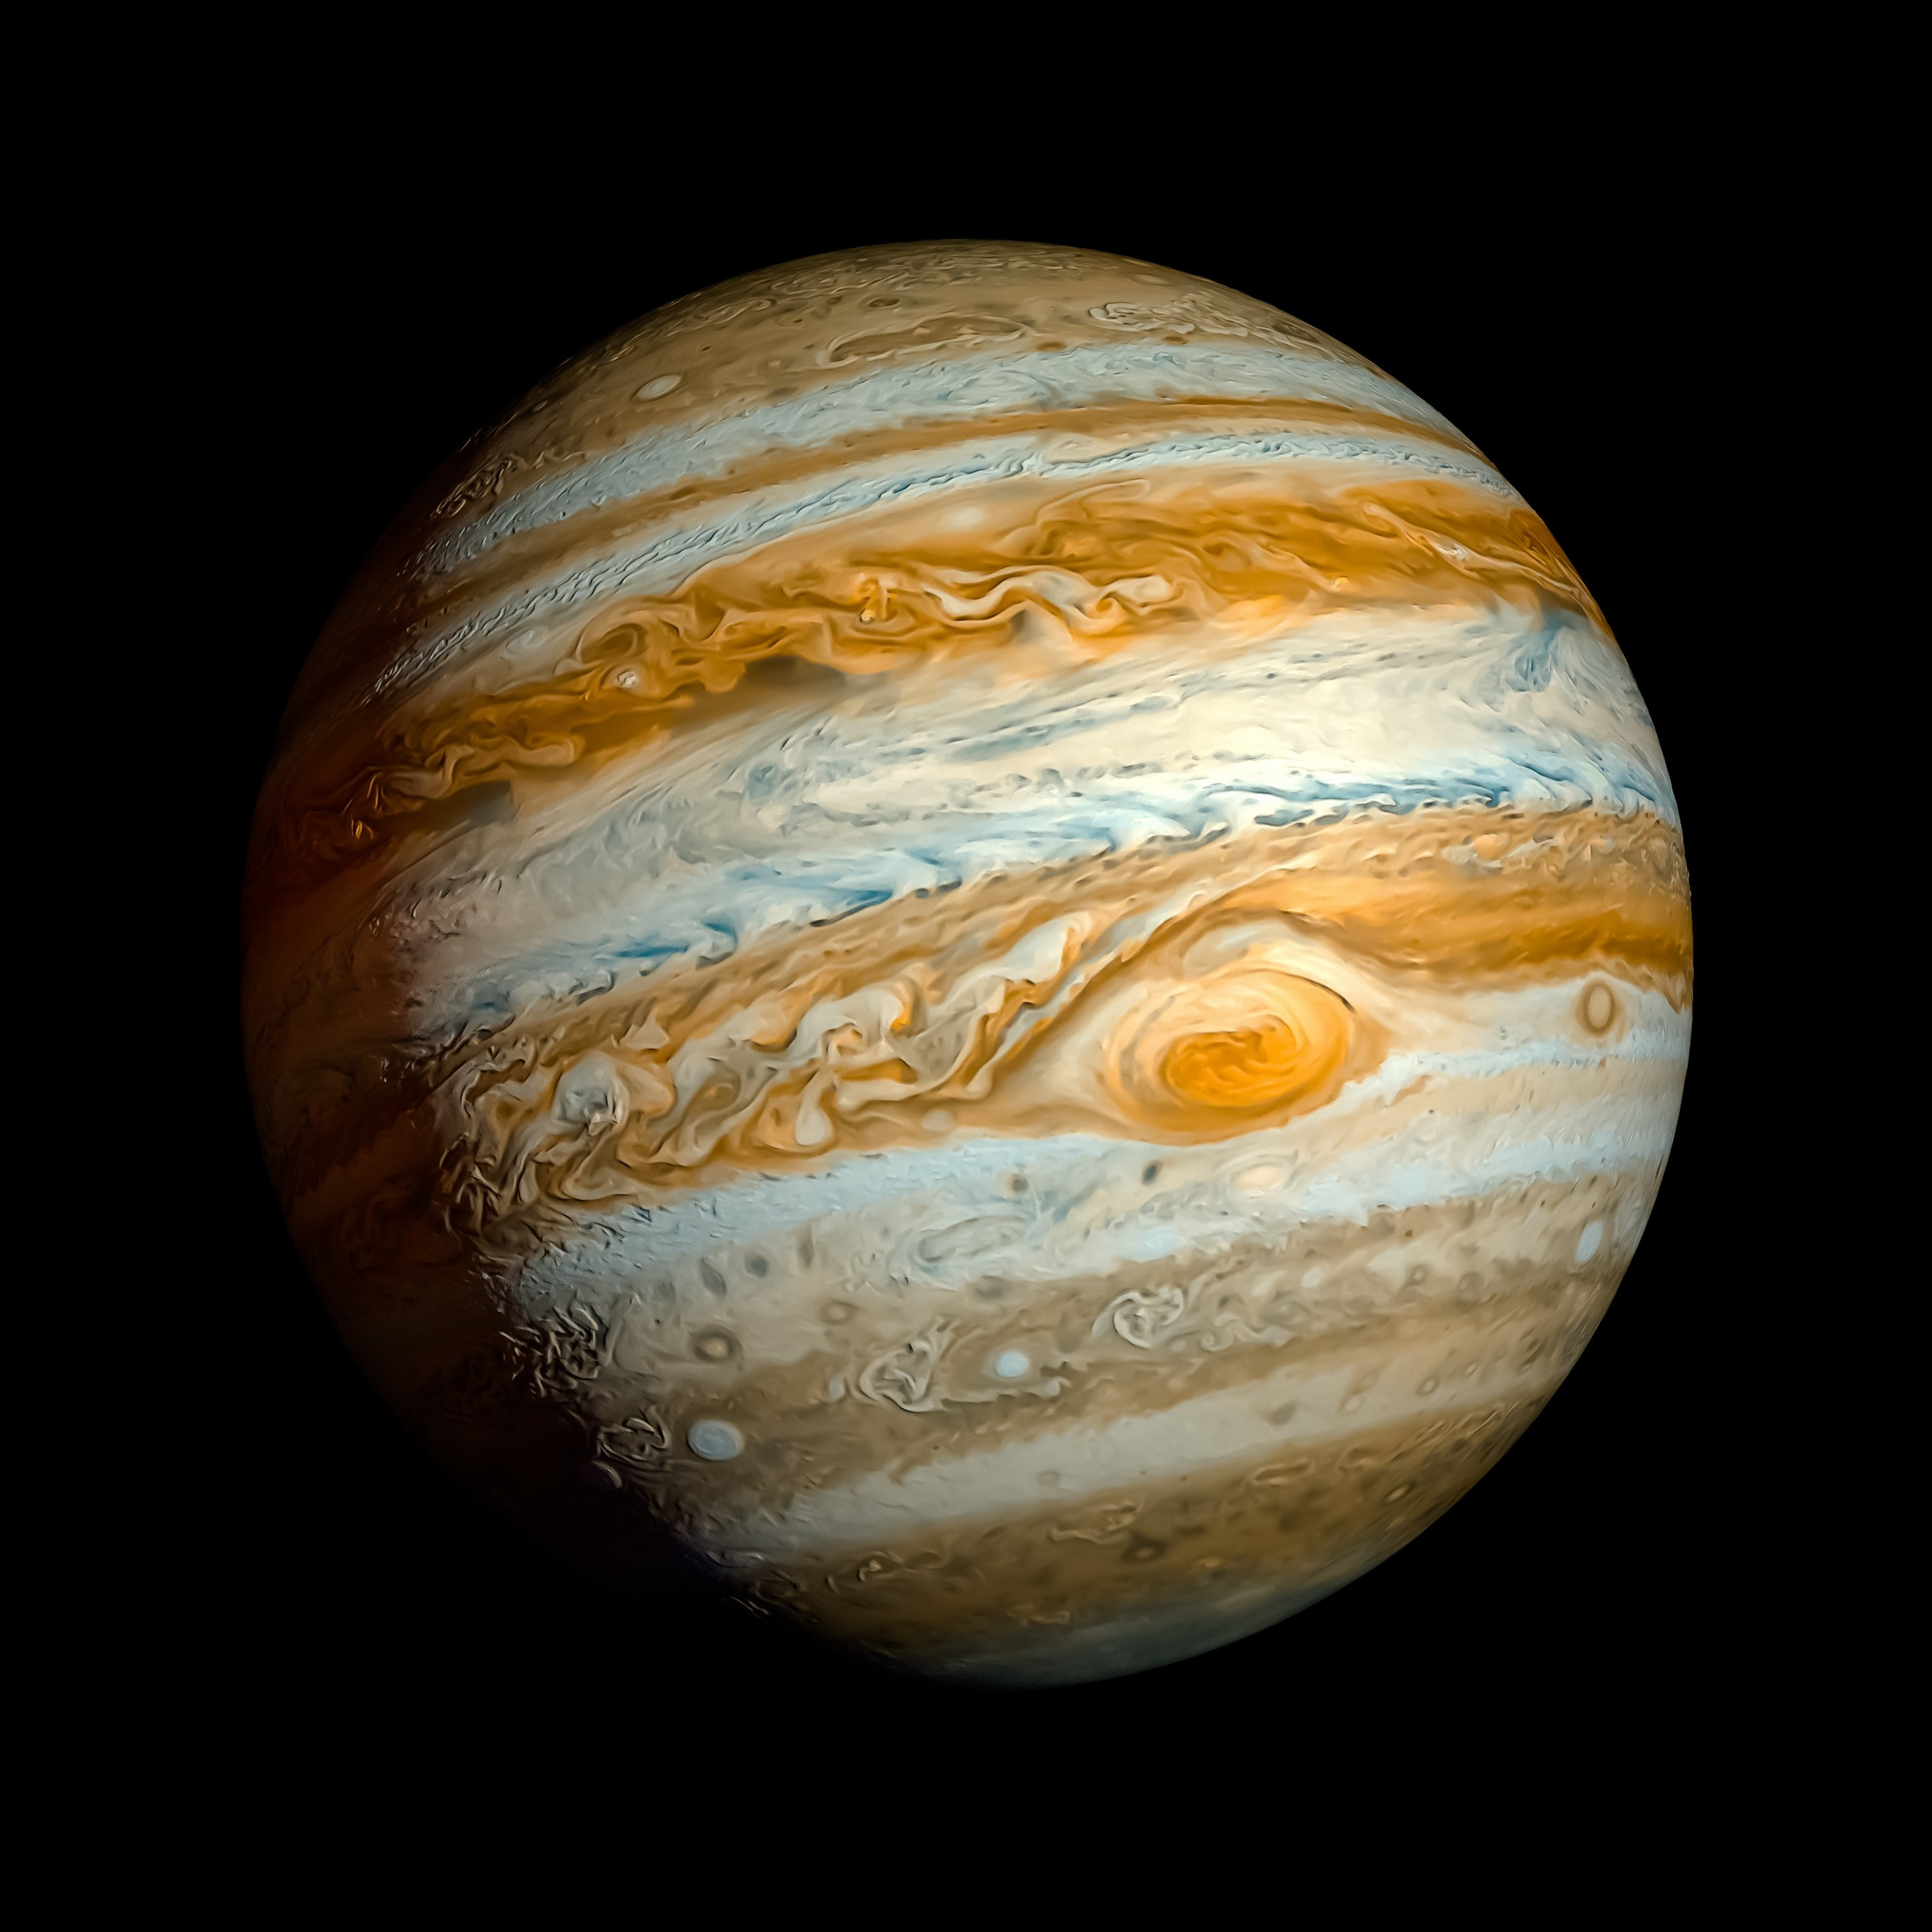
\includegraphics[width=\textwidth]{Jupiter}
	\end{subfigure}
	\begin{subfigure}[b]{0.45\textwidth}
		\caption{Earth at night}\label{fig:Earth}
		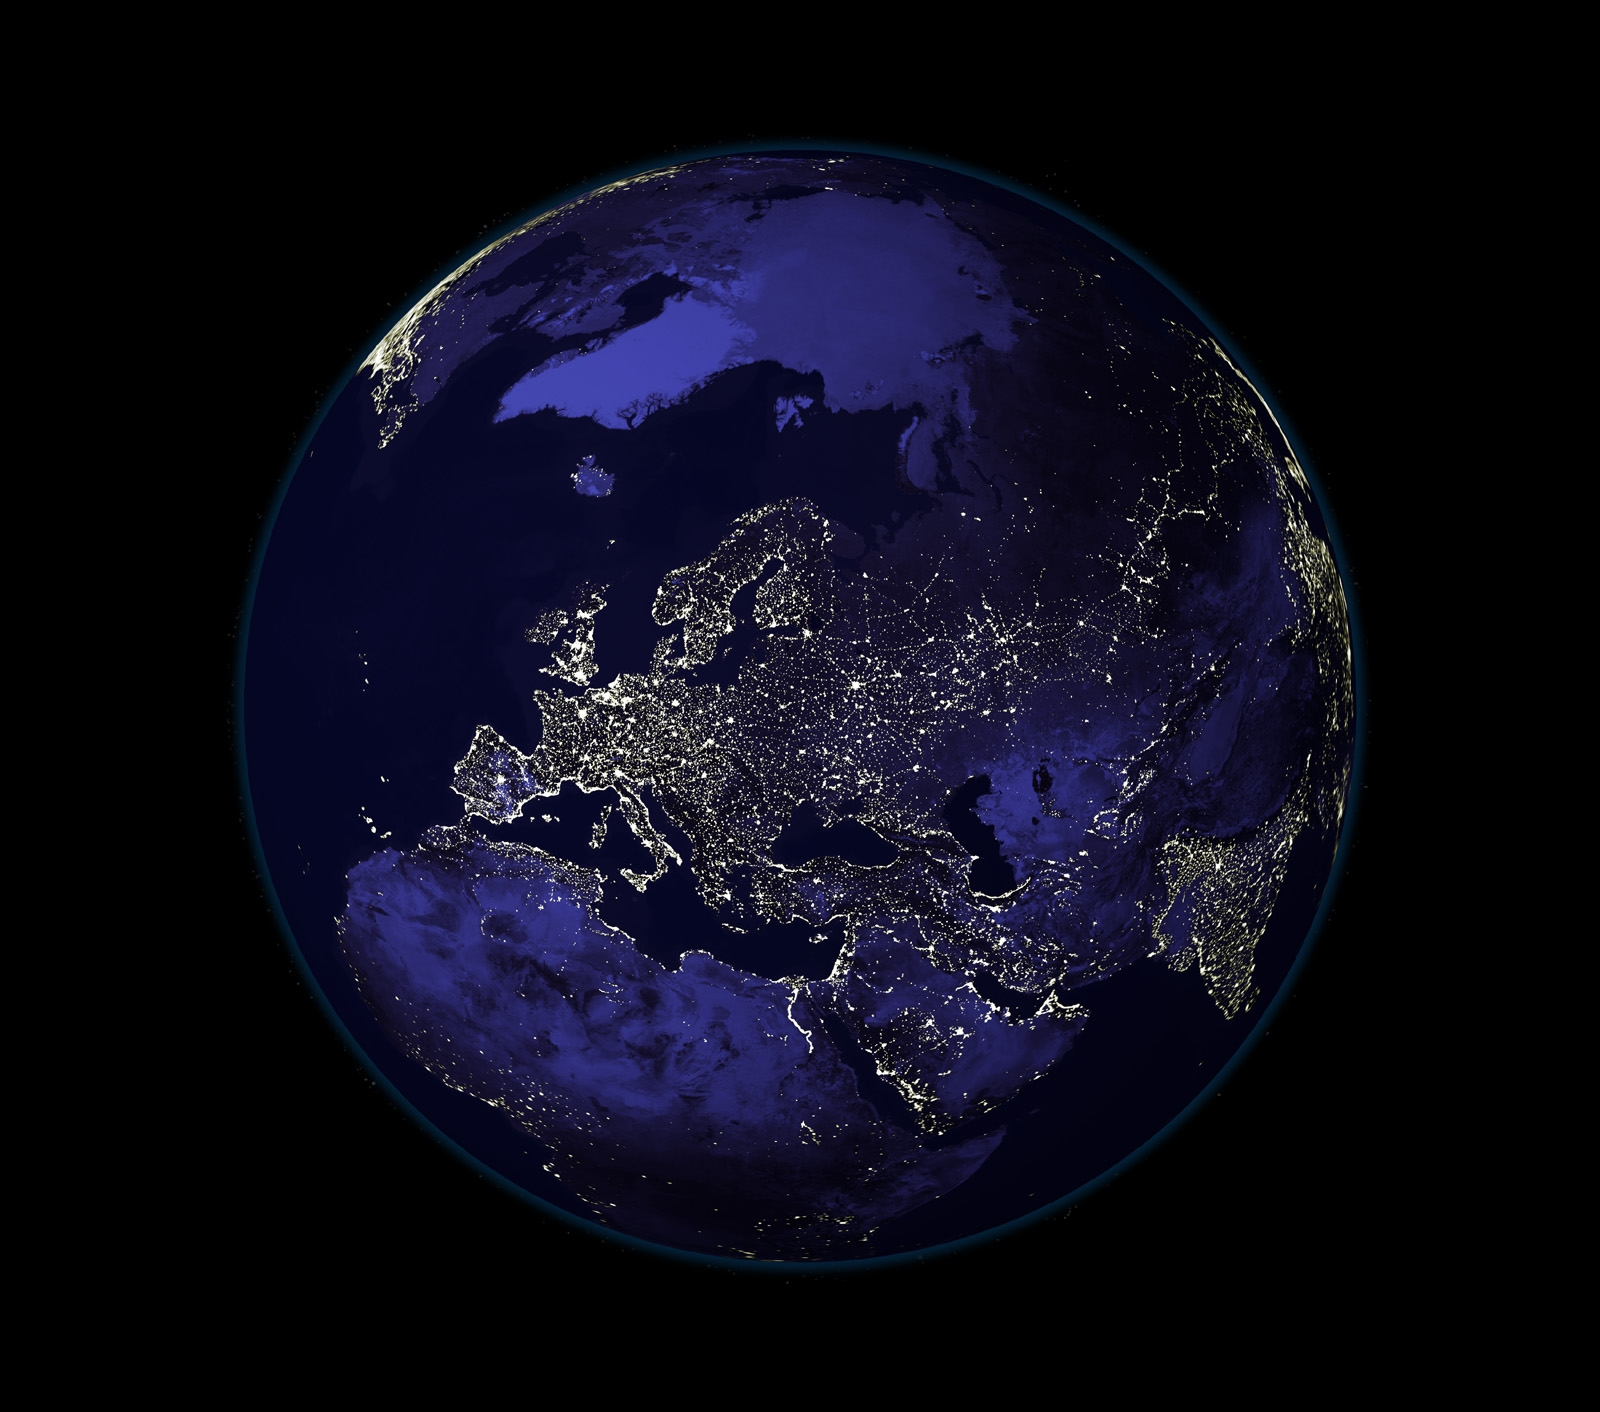
\includegraphics[width=\textwidth]{Tellus}
	\end{subfigure}
\end{figure}

Figure \ref{fig:P:Life} shows how we can constrain the probability of Life.  Our Theory should be able to explain the differences in Figure \ref{fig:Jupiter:Tellus}.

\begin{figure}[H]
	\caption{Rate of abiogenesis in a prebiotic environment as a function of its physical and chemical conditions}\label{fig:P:Life}
	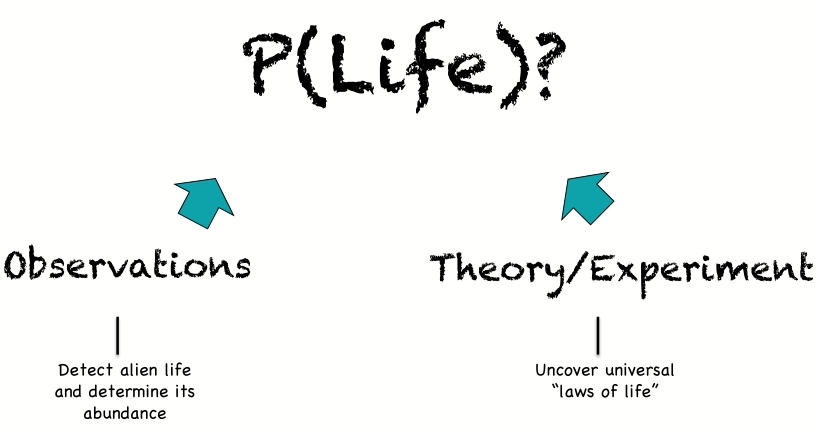
\includegraphics[width=0.9\textwidth]{P_Life}
\end{figure}

''Base metals can be transmuted into gold by stars, and by intelligent beings who understand the processes that power stars, and by nothing else in the universe''--David Deutsch\cite{deutsch2011beginning}.

We want a theory that allows us to understand the diversity of Figure \ref{fig:Earth}.

\section{Exoplanets}

\subsection{The Habitable Zone}

\cite{fujii2018exoplanet}
\cite{villanueva2015unique}
\cite{kasting1993habitable}
\cite{kopparapu2013habitable}
\cite{nasa2019Explonet}

\subsection{Exoplanet Atmospheric Characterization}

\cite{sagan1993search}
\cite{kaltenegger2017characterize}
\cite{fujii2018exoplanet}
\cite{nasa2019Explonet}
\cite{robinson2011earth}
\cite{marois2010images}
\cite{greenbaum2018gpi}
\cite{deming2013infrared}
\cite{knutson2007map}

\section{What is Life?}

\subsection{Constraining the Definition of Life}

\cite{schrodinger1944life}

\subsection{Weird Life}

\cite{hollants2011life}

\cite{kim2001life}

\cite[Chapter 6: Why Water? Toward More Exotic Habitats ]{board2007limits}

\cite{cejkova2014dynamics}

\section{Abstract and general Models for Life}

\cite{trifonov2011vocabulary}

\cite{cronin2016beyond}

\section{The Multiple Origins of Life}

\subsection{The Argument}

\subsection{Reversing the Arrow of Time}

\subsection{The Theory of the Adaptive Arrow of Time}

\cite{rockmore2018cultural}

\subsection{Evolutionary Agents}

\section{Evolutionary Computation}

\cite{mitchell1998introduction}
\cite{eiben2003introduction}
\cite{holland1992adaptation}
\cite{forrest1993genetic}
\cite{ma2014novo}
\cite{marshall2014evolution}


\section{Scaling}

\cite{anderson2013altered}
\cite{damuth1981population}
\cite{enquist1998allometric}
\cite{enquist2012land}
\cite{marquet2005scaling}
\cite{schmidt1984scaling}
\cite{tucker2014evolutionary}
\cite{west1997general}

\section{Energy}

\cite{odum1976energy}
\cite{odum1983systems}
\cite{schmidt1997animal}
\cite{brown2004toward}
\cite{sibly2012metabolic}
\cite{ernest2003thermodynamic}
\cite{savage2004predominance}
\cite{dell2011systematic}
\cite{kempes2017thermodynamic}

% end of text 

% glossary
\printglossaries

% bibliography go here
 
\bibliographystyle{unsrt}
\addcontentsline{toc}{section}{Bibliography}
\bibliography{origins,wikipedia}

\end{document}
